\section{Pressurized hollow sphere}
\paragraph{}
The problem is a pressurized hollow sphere subjected to internal pressure. The geometry of the problem is described in fig.\ref{oct_fig:ex_pre-hollow-sphere}. 

\begin{figure}[h!]
  \centering
  \scalebox{1}{\includegraphics{octree/ex_images/oct_ex_image021.jpg}}
  \caption{Pressurized hollow sphere}
  \label{oct_fig:ex_pre-hollow-sphere}
\end{figure}

\paragraph{}
In the example, the external pressure is set to be zero so that only the internal one is considered. $a=20, b=150, p_a = 10,p_b = 0, E=200,\nu=0.3$. Instead of a quarter of a hollow sphere, a cubic with a spherical hole is analysed. Displacement boundary condition is applied on all of the boundary surface. First order tetrahedral element is adopted to calculated the displacement and stress and compared to the exact solution as in eq.~\ref{oct_eq:ex_hollow_sphere_ana_sol} in spherical coordinate.

\begin{subequations}
\begin{align}
  u & = \frac{1}{2E(b^3-a^3)R^2}\left\{ 2(p_aa^3-p_bb^3)(1-2\nu)R^3+(p_a-p_b)(1+\nu)b^3a^3\right\}\\
  \sigma_{RR} & = \frac{p_aa^3-p_bb^3}{b^3-a^3} - \frac{(p_a-p_b)b^3a^3}{(b^3-a^3)R^3}\\
  \sigma_{\theta\theta} & = \frac{p_aa^3-p_bb^3}{b^3-a^3} + \frac{(p_a-p_b)b^3a^3}{2(b^3-a^3)R^3}\\
  \sigma_{\phi\phi} & = \sigma{\theta\theta}
  \label{oct_eq:ex_hollow_sphere_ana_sol}
\end{align}
\end{subequations}

\paragraph{}
The tensor transformation from spherical coordinate to cartesian coordinate can be written as eq.\~ref{eqn:transformation} with according to fig.~\ref{octree_fig:oct_ex_hollow_sphere_tran}.
\begin{subequations}
  \begin{align}
    \begin{bmatrix}
      S_{xx} & S_{xy} & S_{xz} \\
      S_{xy} & S_{yy} & S_{yz} \\
      S_{xz} & S_{yz} & S_{zz} \\
    \end{bmatrix} = T\begin{bmatrix}
      S_{RR} & S_{R\theta} & S_{R\phi} \\
      S_{R\theta} & S_{\theta\theta} & S_{\theta\phi}\\
      S_{R\phi} & S_{\theta\phi} & S_{\phi\phi} \\
    \end{bmatrix} T^T\\
  T = 
\begin{bmatrix}
\sin\theta\cos\phi & \cos\theta\cos\phi & -\sin\phi \\
\sin\theta\sin\phi & \cos\theta\sin\phi & \cos\phi  \\
\cos\theta & -\sin\theta & 0 \\
\end{bmatrix}
\end{align}
\label{eqn:transformation}
\end{subequations}

\begin{figure}[h!]
    \centering
    \scalebox{1}{\includegraphics{octree/ex_images/oct_ex_tran.png}}
    \caption{Coordinate transformation}
    \label{octree_fig:oct_ex_hollow_sphere_tran}
  \end{figure}
  
\paragraph{}
In the example, $a = 10,b = 50, E=20,\nu = 0.2,P_a = 10$. For simplification, only a quarter of the sphere is analysed as shown in fig.~\ref{oct_fig:ex_hollow_sphere_meshP}

\begin{figure}[h!]
  \centering
  \scalebox{0.5}{\includegraphics{octree/ex_images/oct_ex_mesh.png}}
  \caption{Mesh of the problem}
  \label{oct_fig:ex_hollow_sphere_meshP}
\end{figure}

Stress boundary in Eq.~\ref{oct_eq:ex_sphere_hole_bond_str} condition is applied on two spherical surfaces.
\begin{subequations}
    \begin{align}
    \sigma_{RR}(R=a,\phi,\theta) & = \frac{p_aa^3-p_bb^3}{b^3-a^3} - \frac{(p_a-p_b)b^3a^3}{(b^3-a^3)R^3}\\
    u_z(x,y,0) &= 0\\
    u_y(x,0,z) & = 0 \\
    u_x(0,y,z) & = 0
  \end{align}
\label{oct_eq:ex_sphere_hole_bond_str}
\end{subequations}

The convergence study is plotted in Fig.~\ref{oct_fig:ex_hollow_sphere_conv}
\begin{figure}[h!]
    \centering
    \scalebox{0.5}{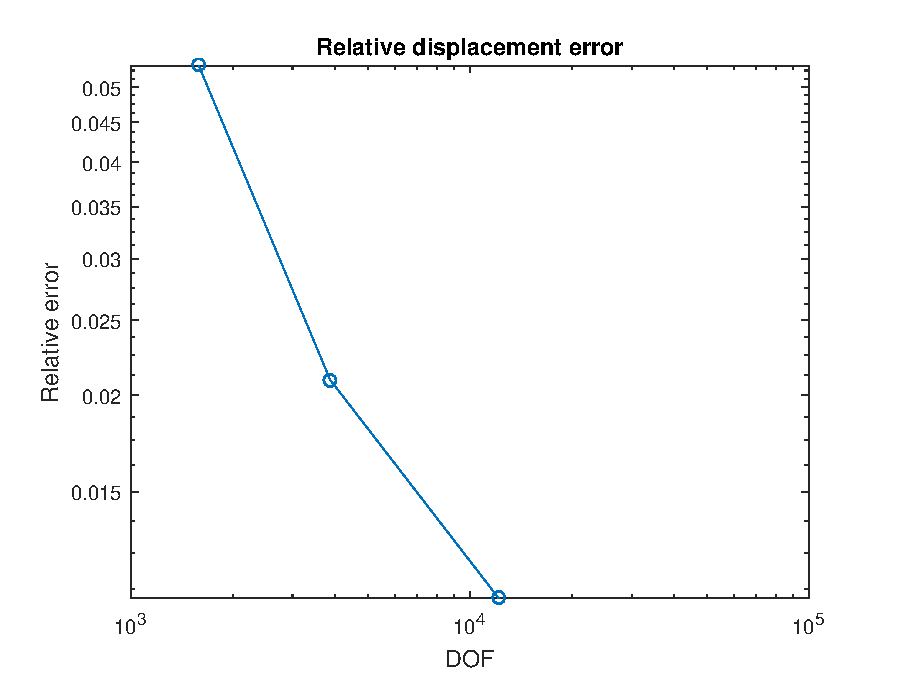
\includegraphics{octree/ex_images/ex_sphere_hole_conv.eps}}
    \caption{Convergence of displacement error}
    \label{oct_fig:ex_hollow_sphere_conv}
  \end{figure}